\documentclass{article}

\usepackage{float}
\usepackage{mathtools}
\usepackage{graphicx}
\usepackage{geometry}
\usepackage{subfig}
\usepackage[table]{xcolor}
\usepackage{bera}
\usepackage{listings}
\usepackage{verbatim} 
\usepackage{fancyvrb}
\usepackage{algorithm}
\usepackage{algorithmic}
\usepackage{hyperref}
\usepackage{tikz}
    \usetikzlibrary{positioning}
\usepackage{xepersian}



\geometry{margin=20mm}

\settextfont{B Nazanin}

\graphicspath{ {./pics/} }

\definecolor{codegreen}{rgb}{0,0.6,0}
\definecolor{codegray}{rgb}{0.5,0.5,0.5}
\definecolor{codepurple}{rgb}{0.58,0,0.82}
\definecolor{backcolour}{rgb}{0.95,0.95,0.92}


\renewcommand{\algorithmicif}{\textbf{اگر}}
\renewcommand{\algorithmicthen}{\textbf{آنگاه}}
\renewcommand{\algorithmicelse}{\textbf{وگرنه}}
\renewcommand{\algorithmicprint}{\textbf{چاپ کن}}
\renewcommand{\algorithmicendif}{\textbf{پایان شرط}}

\lstdefinestyle{mystyle}{
    backgroundcolor=\color{backcolour},   
    commentstyle=\color{codegreen},
    keywordstyle=\color{blue},
    numberstyle=\tiny\color{codegray},
    stringstyle=\color{codepurple},
    basicstyle=\ttfamily\footnotesize,
    breakatwhitespace=false,         
    breaklines=true,                 
    captionpos=b,                    
    keepspaces=true,                 
    numbers=left,                    
    numbersep=5pt,                  
    showspaces=false,                
    showstringspaces=false,
    showtabs=false,                  
    tabsize=2
}

\lstset{style=mystyle}

%\lstdefinestyle{}{
%captiondirection=RTL,language=matlab
%}

\lstdefinestyle{verilog}{
captiondirection=RTL,language=Verilog
}
%\definecolor{vgreen}{RGB}{104,180,104}
%\definecolor{vblue}{RGB}{49,49,255}
%\definecolor{vorange}{RGB}{255,143,102}
%
%\lstdefinestyle{verilog-style}
%{
%    language=Verilog,
%    basicstyle=\small\ttfamily,
%    keywordstyle=\color{vblue},
%    identifierstyle=\color{black},
%    commentstyle=\color{vgreen},
%    numbers=left,
%    numberstyle=\tiny\color{black},
%    numbersep=10pt,
%    tabsize=8,
%    moredelim=*[s][\colorIndex]{[}{]},
%    literate=*{:}{:}1
%}
%\makeatletter
%\newcommand*\@lbracket{[}
%\newcommand*\@rbracket{]}
%\newcommand*\@colon{:}
%\newcommand*\colorIndex{%
%    \edef\@temp{\the\lst@token}%
%    \ifx\@temp\@lbracket \color{black}%
%    \else\ifx\@temp\@rbracket \color{black}%
%    \else\ifx\@temp\@colon \color{black}%
%    \else \color{vorange}%
%    \fi\fi\fi
%}
%\makeatother

\def\lstlistingname{کد}
\lstset{numberstyle=\tiny\lr}

\begin{document}

\begin{titlepage}
   \begin{center}
   \Large
       \vspace*{1cm}

       \textbf{گزارش پروژه‌ی درس معماری کامپیوتر}

       \vspace{0.5cm}
      پیاده‌سازی جمع‌کننده و ضرب کننده‌ها        
      
       \vspace{1.5cm}
       {علی بهمنیار - ۹۸۲۳۰۱۸}
       \vfill
 
       \vspace{0.8cm}
     	\begin{figure}[H]%
	   	 	\centering
	    	\subfloat{{
\includegraphics[height=4cm]{logo_ee}}}
	    	\quad
	   	 	\subfloat{{
\includegraphics[height=4cm]{logo_uni}}}
		\end{figure}
            
       دانشکده‌ی مهندسی برق\\
       دانشگاه صنعتی امیرکبیر\\
       دی ماه ۱۴۰۱       
   \end{center}
\end{titlepage}

\pagebreak
\tableofcontents
\pagebreak

\section{جمع‌کننده‌ها}
\subsection{\lr{Ripple Adder}}
این جمع کننده، ساده‌ترین نوع جمع‌کننده می‌باشد و طراحی نسبتاً ساده‌ای دارد. شمای کلی این طراحی در شکل \ref{fig:rip-car-schem} مشخص است:
\begin{figure}[H]
\centering
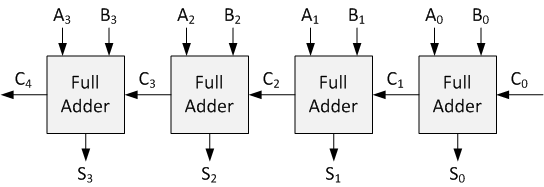
\includegraphics[width=12cm]{ripple-carry-adder-schematic}
\caption{شماتیک کلی جمع‌کننده‌ی \lr{Ripple Adder}}
\label{fig:rip-car-schem}
\end{figure}
\noindent
در این طراحی هر دو بیت توسط یک \lr{Full Adeer} با یکدیگر جمع شده، سپس بیت \lr{carry} حاصل به عنوان بیت \lr{carry} ورودی به \lr{Full Adder} بعدی داده شده تا دو بیت بعدی با یکدیگر جمع شده و این فرآیند تکرار می‌شود تا حاصل جمع نهایی ایجاد شود. \\
در این جمع‌کننده هر \lr{Full Adder} باید منتظر جواب واحد قبلی خود بماند و بنابراین برای ایجاد پاسخ نهایی سیگنال باید به ترتیب از تمامی \lr{Full Adder}ها عبور کند. به این دلیل این جمع‌کننده سرعت عملرد نسبتاً پایینی دارد.\\
پس از پیاده‌سازی این جمع‌کننده، شماتیک \lr{RTL} آن به صورت شکل \ref{fig:rip-car-rtl} می‌باشد:
\begin{figure}[H]
\centering
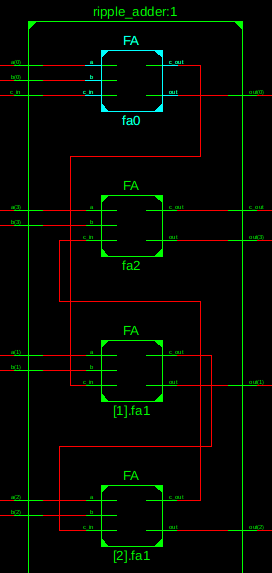
\includegraphics[height=10cm]{ripple-carry-adder-rtl}
\caption{شماتیک \lr{Ripple Adder}}
\label{fig:rip-car-rtl}
\end{figure}
\noindent
این جمع‌کننده به صورت پارامتری برای $N$ بیت پیاده‌سازی شده و تعداد بیت‌های آن توسط پارامتر $N$ ماژول قابل تنظیم است.
\pagebreak
\subsection{\lr{Carry-Lookahead Adder}}
این جمع‌کننده نسبت به جمع‌کننده‌ی قبلی سرعت بیش‌تری دارد، اما همچنین ساختار آن نیز پیچیده‌تر است. ساختار کلی این جمع‌کننده در شکل \ref{fig:cla-schem} مشخص است:
\begin{figure}[H]
\centering
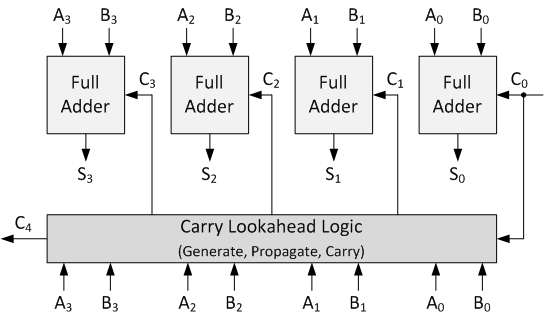
\includegraphics[width=11cm]{carry_lookahead_adder}
\caption{شماتیک کلی جمع‌کننده‌ی \lr{Carry-Lookahead}}
\label{fig:cla-schem}
\end{figure}
\noindent
در جمع‌کننده‌ی \lr{Ripple Carry} عامل اصلی تأخیر این است که هر واحد باید منتظر نتیجه‌ی بیت \lr{carry} واحد قبلی بماند، در این پیاده‌سازی برای برطرف کردن این مشکل می‌توان بیت‌های \lr{carry} را برای هر \lr{Full Adder} به صورت جداگانه توسط یک بخش مجزا محاسبه کرد. این کار باعث می‌شود تا پیچیدگی مدار بیش‌تر شود ولی سرعت انجام جمع را به طور قابل ملاحظه‌ای افزایش می‌دهد.
پس از پیاده‌سازی این جمع‌کننده، بخشی از شماتیک \lr{RTL} آن به صورت شکل \ref{fig:cla-adder-rtl} می‌باشد، از این شماتیک نیز پیچیدگی بیش‌تر مدار نسبت به راه‌حل قبلی مشخص است:
\begin{figure}[H]
\centering
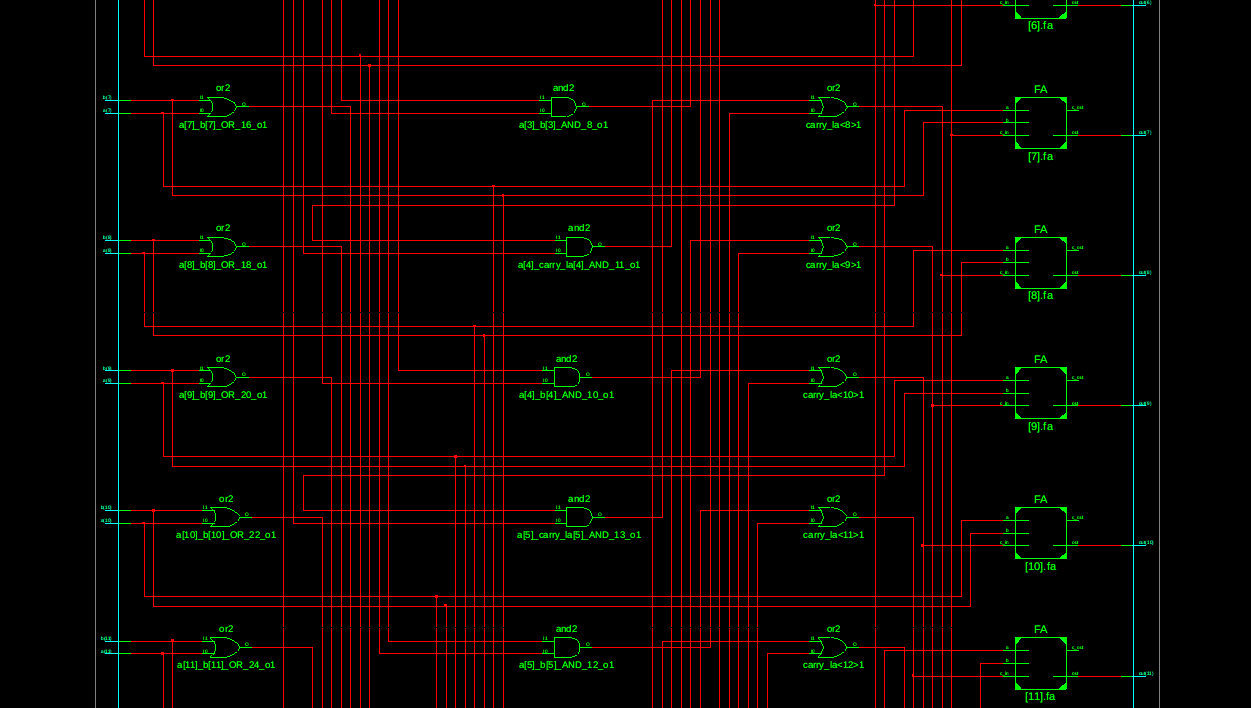
\includegraphics[width=10cm]{cla-adder-rtl}
\caption{شماتیک \lr{Carry-Lookahead Adder}}
\label{fig:cla-adder-rtl}
\end{figure}
\noindent
این جمع‌کننده به صورت پارامتری برای $N$ بیت پیاده‌سازی شده و تعداد بیت‌های آن توسط پارامتر $N$ ماژول قابل تنظیم است.

\begin{LTR}
\begin{lstlisting}[caption={\rl{پیاده‌سازی \lr{Carry-Lookahead}}​},label=code:cla,style=verilog]
assign carry_la[j] = (a[j-1] & b[j-1]) | ((a[j-1] | b[j-1]) & carry_la[j-1]);
\end{lstlisting}
\end{LTR}
\noindent
پیاده‌سازی \lr{Carry-Lookahead} در کد \ref{code:cla} مشخص است؛ در دو صورت بیت \lr{carry} می‌بایست ۱ باشد: یا هر دو بیت ورودی ۱ باشند، یا یکی از بیت‌های ورودی به همراه بیت \lr{carry} قبلی ۱ باشند.

\pagebreak
\subsection{\lr{Carry Select Adder}}
در راهکار قبلی سرعت محاسبه بهبود یافت اما همچنان برای محاسبه‌ی هر یک از بیت‌های \lr{carry} می‌بایست منتظر خروجی بیت \lr{carry} قبلی در مدار \lr{carry-lookahead} بمانیم، به عبارت دیگر انتشار سیگنال در مدار \lr{carry-lookahead} همچنان زمان‌بر است.\\
راهکار دیگر این است که کل عملیات جمع را به دسته‌های $n$ بیتی تقسیم کنیم و عملیات جمع را ابتدا به ازای هر دو بیت کری $0$ و $1$ انجام دهیم، سپس بعد از مشخص شدن بیت کری صحیح با استفاده از یک مالتی‌پلکسر آن را انتخاب کنیم. شمای کلی این راهکار در شکل \ref{fig:carry-select-schematic} مشخص است.
\begin{figure}[H]
\centering
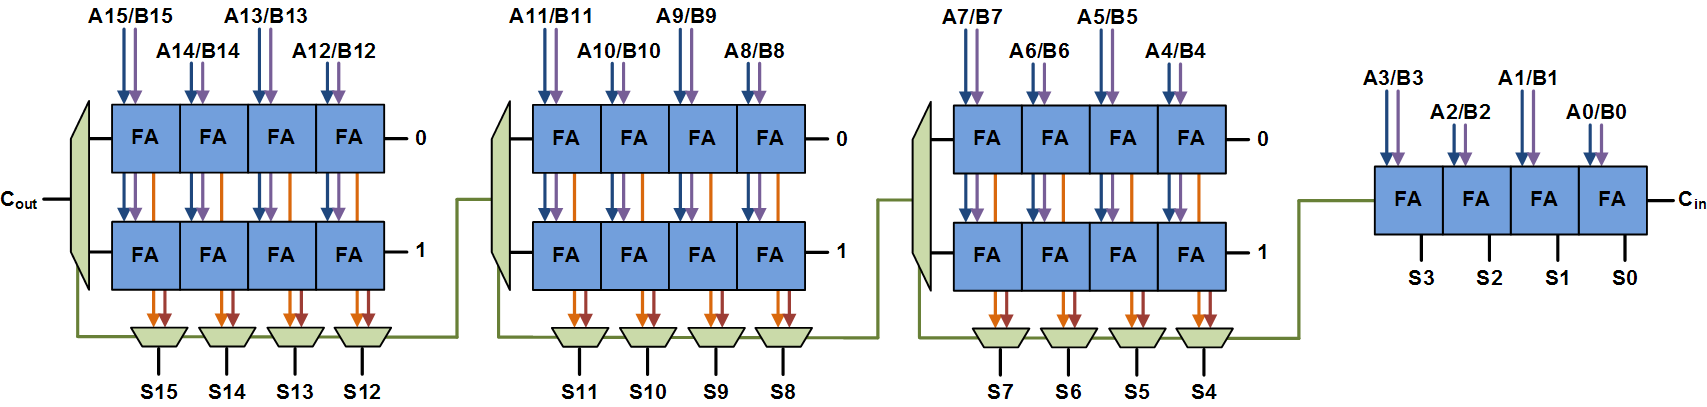
\includegraphics[width=16cm]{Carry-select-adder}
\caption{شماتیک کلی \lr{Carry Select Adder}}
\label{fig:carry-select-schematic}
\end{figure}
\noindent
هر یک از بلوک‌های ۴ تایی در واقع یک \lr{ripple adder} هستند. بهینه‌ترین سایز زیر بلوک برای یک جمع $n$ بیتی نیز برابر با
$\lfloor \sqrt{n} \rfloor$
می‌باشد.\\
پس از پیاده‌سازی این جمع‌کننده، بخشی از شماتیک \lr{RTL} آن به صورت شکل \ref{fig:carry-select-adder-rtl} می‌باشد، این جمع‌کننده بیش‌ترین مساحت را اشغال خواهد کرد اما سریع‌ترین جمع‌کننده‌ها نیز خواهد بود.
\begin{figure}[H]
\centering
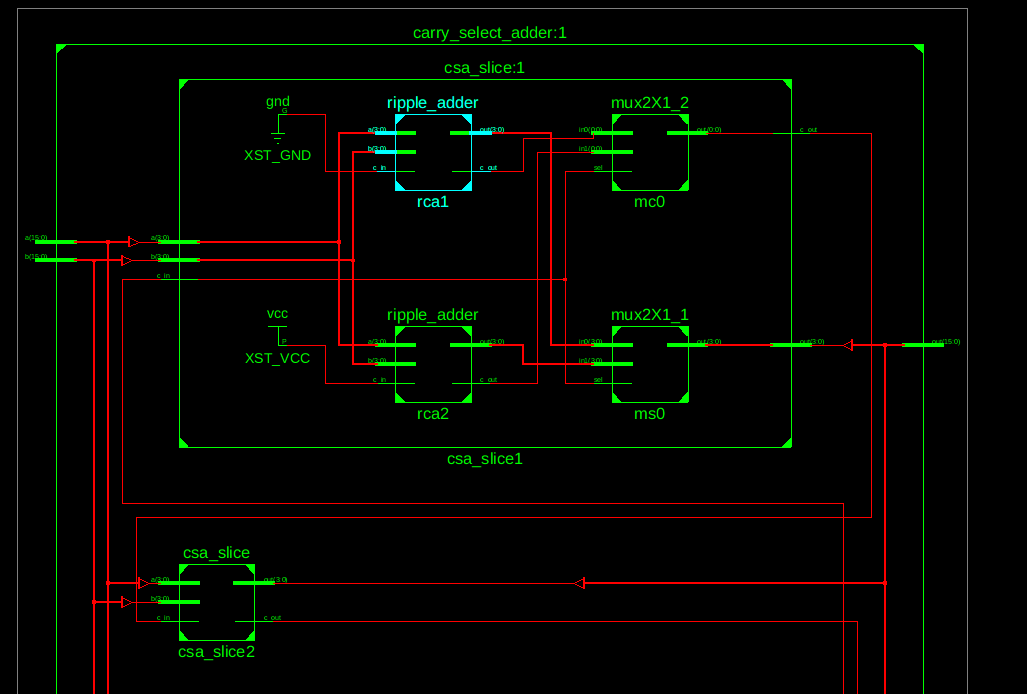
\includegraphics[width=10cm]{carry-select-adder-rtl}
\caption{شماتیک \lr{Carry-select-adder}}
\label{fig:carry-select-adder-rtl}
\end{figure}
\noindent
این جمع‌کننده به صورت ۱۶ بیتی پیاده‌سازی شده است.
\pagebreak
\section{ضرب‌کننده‌ها}
\subsection{\lr{Shift-Add Multiplier}}
این ضرب‌کننده ساده‌ترین نوع ضرب‌کننده می‌باشد، این ضرب‌کننده با استفاده از کلاک در چندین سیکل هربار عملیات ضرب را برای یک بیت انجام داده و سپس حاصل را با خروجی نهایی جمع می‌کند. منطق اصلی این ضرب‌کننده در کد \ref{code:sam} مشخص است:
\begin{LTR}
\begin{lstlisting}[caption={\rl{پیاده‌سازی \lr{Shift-Add Multiplier}}​},label=code:sam,style=verilog]
always @(posedge clk) begin
        if (bn < N) begin
            finished = 0;
            cb = b[bn];

            if (bn == 0) begin
                case (cb)
                    0: res[2*N-1:N] = (a & zero);
                    1: res[2*N-1:N] = (a & one);
                endcase
            end else begin
                case (cb)
                    0: res[2*N:N] = res[2*N-1:N] + (a & zero);
                    1: res[2*N:N] = res[2*N-1:N] + (a & one);
                endcase

            end
            res = res >> 1;
            bn = bn + 1;
        end else begin
            finished = 1;
        end

        out = res;
    end
\end{lstlisting}
\end{LTR}
\noindent
این ضرب‌کننده به صورت پارامتری برای $N$ بیت پیاده‌سازی شده و تعداد بیت‌های آن توسط پارامتر $N$ ماژول قابل تنظیم است.


\subsection{\lr{Array Multiplier}}
جمع‌کننده‌ی \lr{shift-Add} در چندین کلاک کار می‌کند، اما می‌توانیم بدون استفاده از کلاک و تنها با استفاده از یک مدار ترکیبی نیز عملیات ضرب را پیاده‌سازی کنیم، ابتدا می‌توانیم عملیات ضرب را به صورت گسترده مطابق شکل \ref{fig:array_multiplication} بنویسیم:
\begin{figure}[H]
\centering
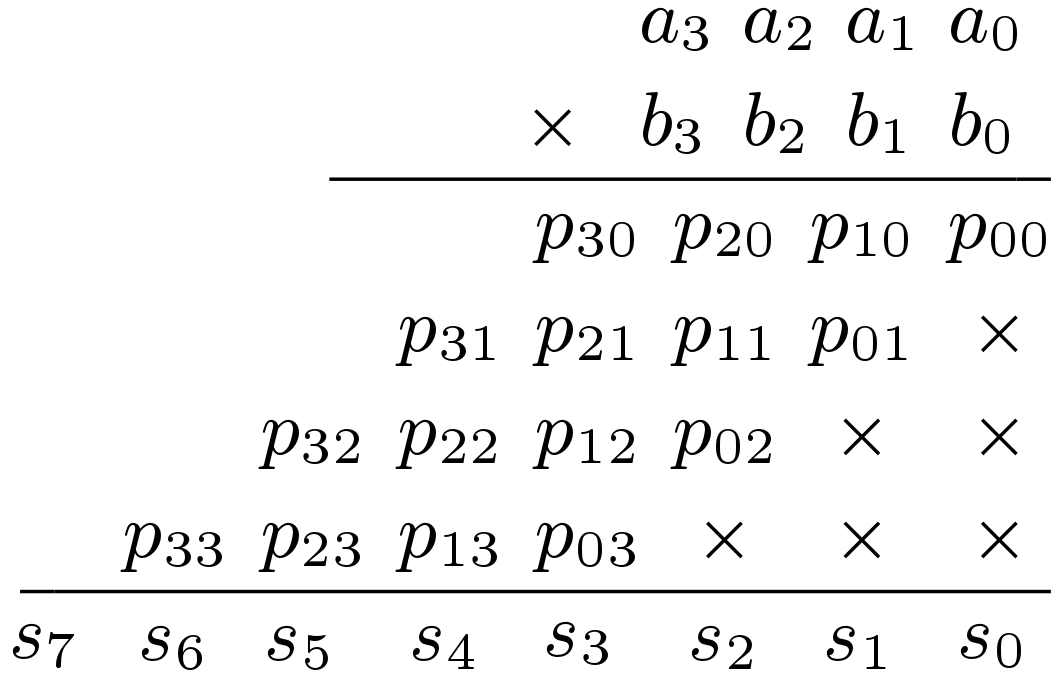
\includegraphics[width=8cm]{array_multiplication}
\caption{نمای گسترده‌ی ضرب دو عدد چهار بیتی}
\label{fig:array_multiplication}
\end{figure}
حال می‌توان تمام عملیات نشان داده‌شده در شکل بالا را توسط یک مدار ترکیبی پیاده‌سازی کرد، شماتیک کلی این مدار به صورت شکل \ref{fig:4-bit-array-multiplier} خواهد بود:
\begin{figure}[H]
\centering
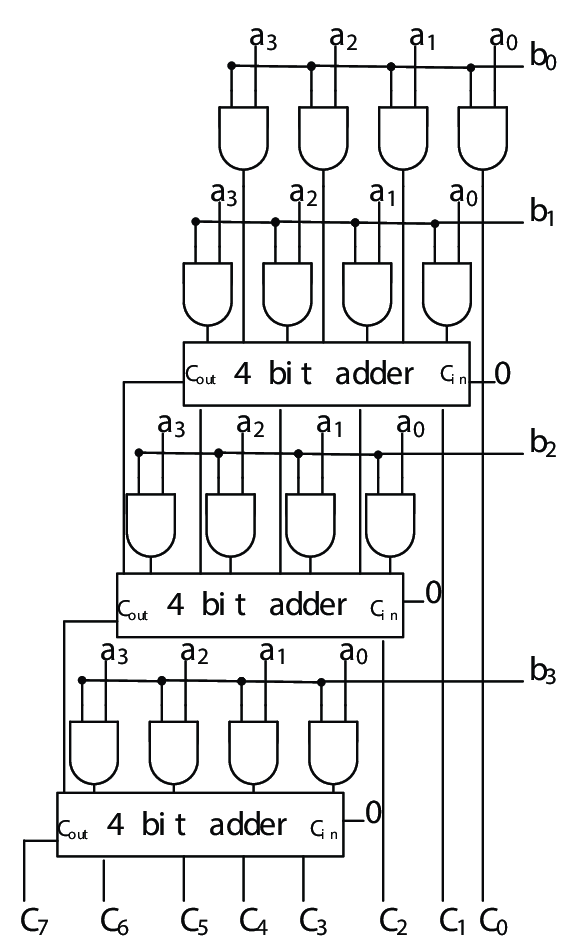
\includegraphics[height=8cm]{4-bit-array-multiplier}
\caption{شماتیک ضرب‌کننده‌ی آرایه‌ای}
\label{fig:4-bit-array-multiplier}
\end{figure}
این ضرب‌کننده به صورت ۴ بیتی پیاده‌سازی شده است.

\subsection{\lr{Carry-Save Multiplier}}
در ضرب کننده‌ی آرایه‌ای می‌بایست همواره منتظر انتشار نتیجه‌ی بیت‌های \lr{carry} بمانیم اما می‌توان عملیات جمع را به صورت دیگری نیز انجام داد، مثال زیر را در نظر می‌گیریم:
\begin{center}
\begin{latin}
\begin{tabular}{c@{\,}c@{\,}c@{\,}c@{\,}c@{\,}c}
 && & 1 & 1 & 1 \\
$\times$ &&&   & 1 & 1 \\
\hline
  & 1 & 0 & 1 & 0 & 1 \\
\end{tabular}
\end{latin}
\end{center}
\noindent
راه دیگر برای انجام ضرب فوق به صورت زیر است:

\begin{center}
\begin{latin}
\begin{tabular}{c@{\,}c@{\,}c@{\,}c@{\,}c@{\,}c}
 & 1 & 1 & 1 \\
$\times$ &   & 1 & 1 \\
\hline
   1 & 2 & 2 & 1 \\
\end{tabular}
\end{latin}
\end{center}
این نمایش نامتداول اما قابل قهم است؛ در واقع این‌جا $2$ نشان دهنده‌ی $10$ است یعنی یک بیت $0$ با بیت کری $1$. بعد از به دست آمدن این نتیجه حال می‌توانیم بیت‌های کری به دست آمده را در مرحله‌ی بعدی جمع کرده و نتیجه‌ی نهایی را به صورت باینری متداول به دست آوریم:
\begin{center}
\begin{latin}
\begin{tabular}{c@{\,}c@{\,}c@{\,}c@{\,}c@{\,}c}
&& 1 & 0 & 0 & 1 \\
+ &&1 &  1 &  &  \\
\hline
  & 1 & 0 & 1 & 0 & 1 \\
\end{tabular}
\end{latin}
\end{center}
\noindent
به عبارت دیگر در جمع \lr{carry-save} ابتدا جمع را حساب کرده سپس نتیجه بیت‌های \lr{carry} را با نتیجه‌ی به دست آمده جمع می‌کنیم.\\
شمای یک جمع‌کننده‌ی \lr{carry-save} در شکل \ref{fig:carry-save-schem} مشخص است:
\begin{figure}[H]
\centering
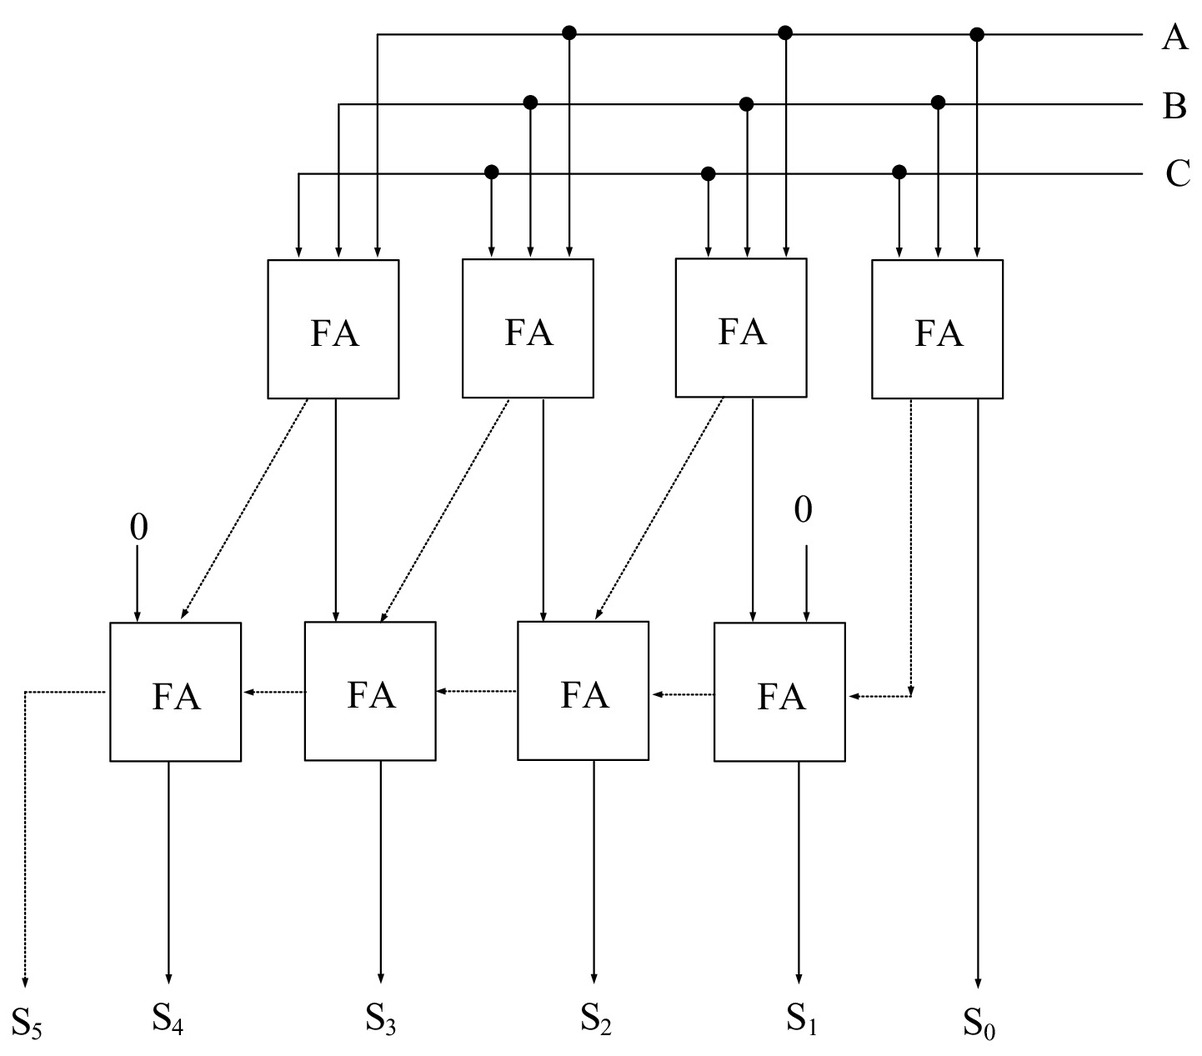
\includegraphics[width=7cm]{carry-save-schem}
\caption{شماتیک \lr{carry-save adder}}
\label{fig:carry-save-schem}
\end{figure}
\noindent
حال می‌توانیم با استفاده از این جمع کننده یک سلول ضرب کننده طراحی کنیم که چهار بیت ورودی می‌گیرد، دو تای آن‌ها را در یکدیگر ضرب کرده نتیجه را با دو بیت دیگر جمع کرده و دو بیت خروجی می‌دهد:
\begin{figure}[H]
\centering
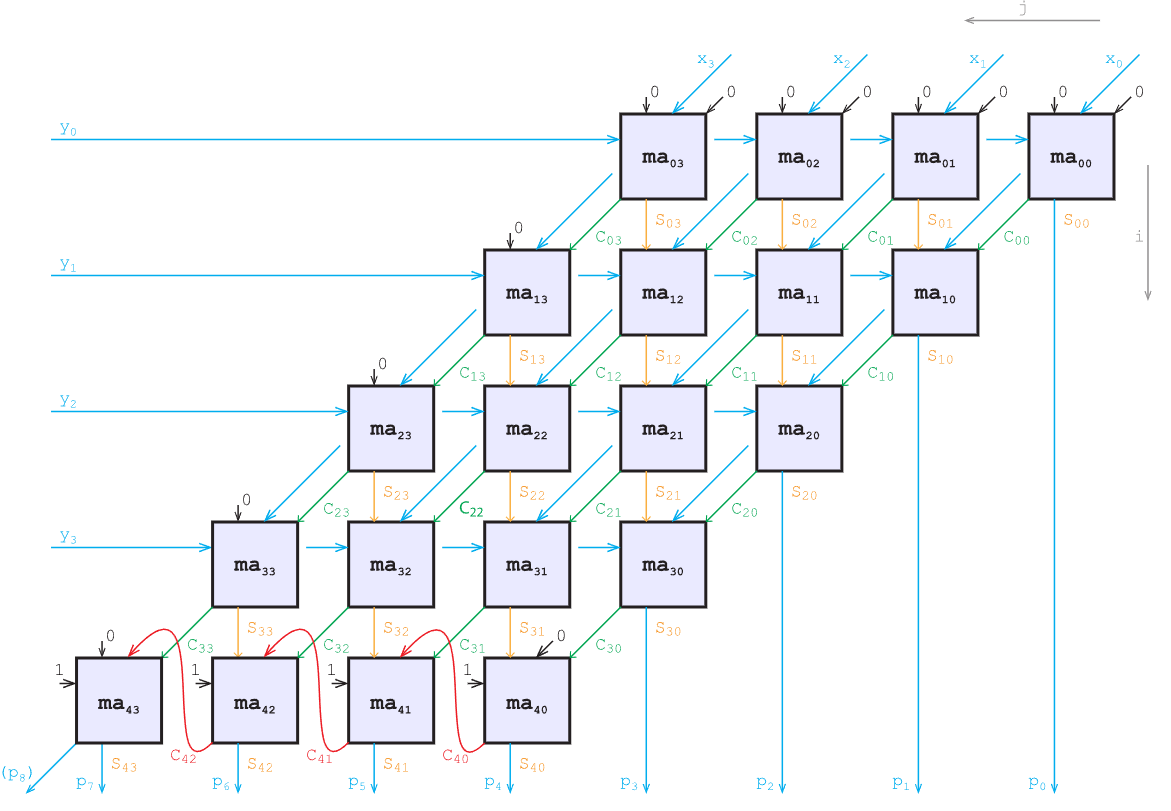
\includegraphics[width=12cm]{carry-save-mul-schem}
\caption{شماتیک \lr{carry-save multiplier}}
\label{fig:carry-save-mul-schem}
\end{figure}
این ضرب‌کننده به صورت ۴ بیتی پیاده‌سازی شده است.

\pagebreak
\appendix
%\renewcommand{\thesection}{پیوست   \alph{section}}
\addcontentsline{toc}{section}{پیوست‌ها}
\section{نتایج شبیه‌سازی‌ها}
\begin{figure}[H]
\centering
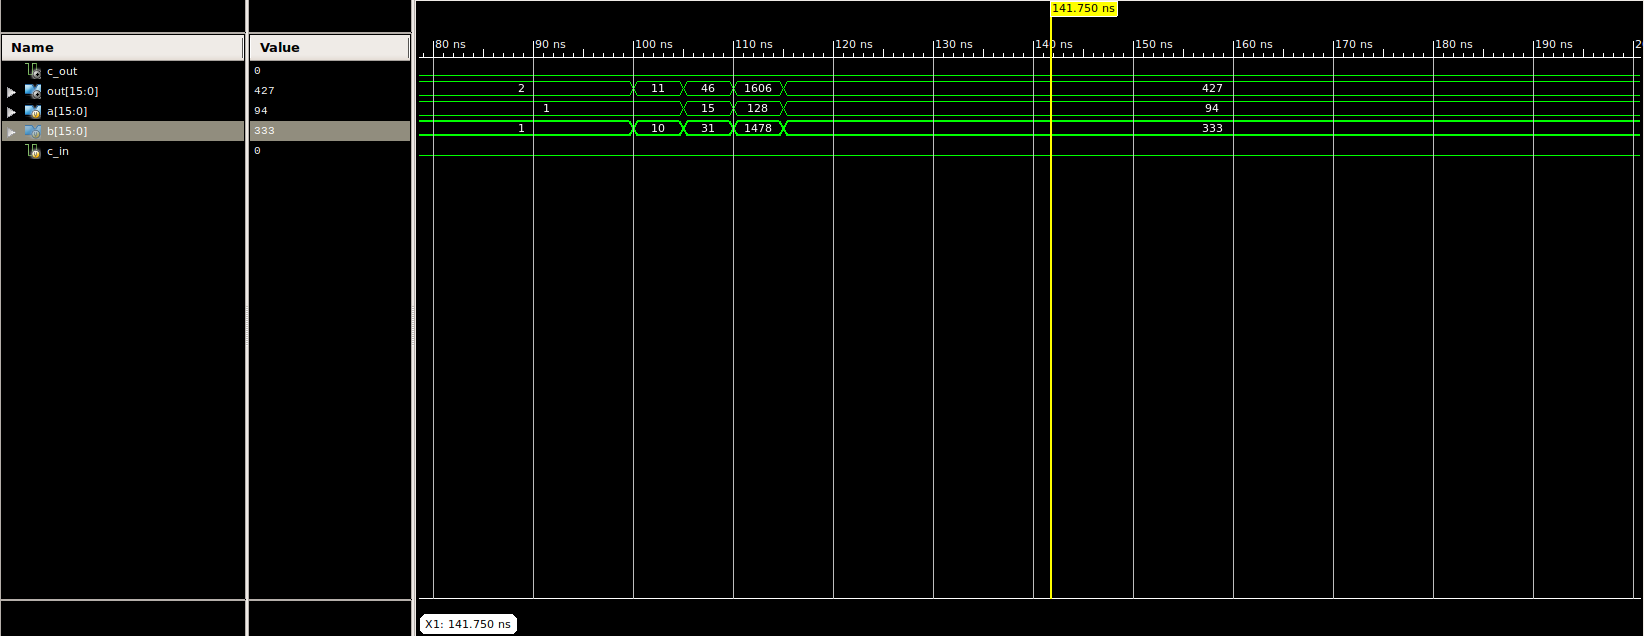
\includegraphics[width=16cm]{adders-tb}
\caption{شبیه‌سازی جمع‌کننده‌ها}
\end{figure}


\begin{figure}[H]
\centering
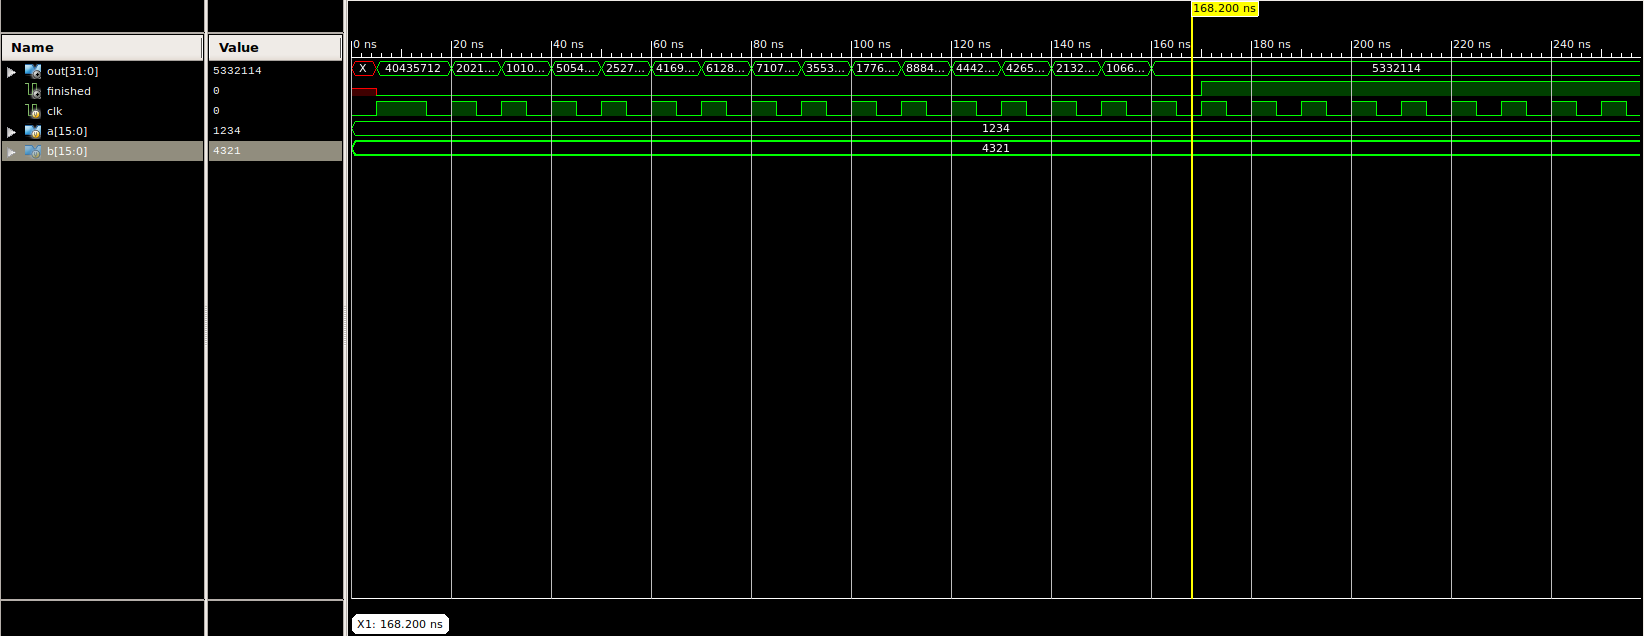
\includegraphics[width=16cm]{shift-add-mul-tb}
\caption{شبیه‌سازی \lr{Shift-Add Multiplier}}
\end{figure}


\begin{figure}[H]
\centering
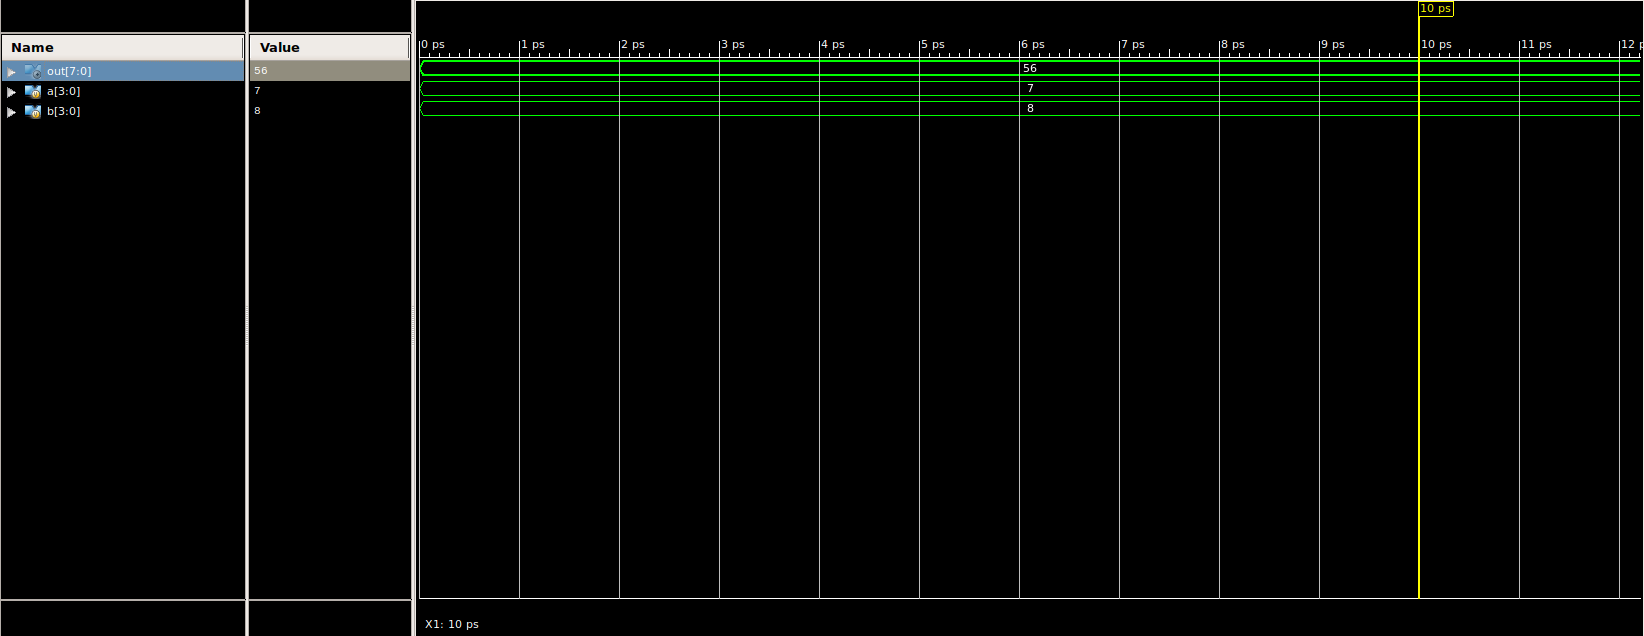
\includegraphics[width=16cm]{array-mul-tb}
\caption{شبیه‌سازی \lr{Array Multiplier}}
\end{figure}

\begin{figure}[H]
\centering
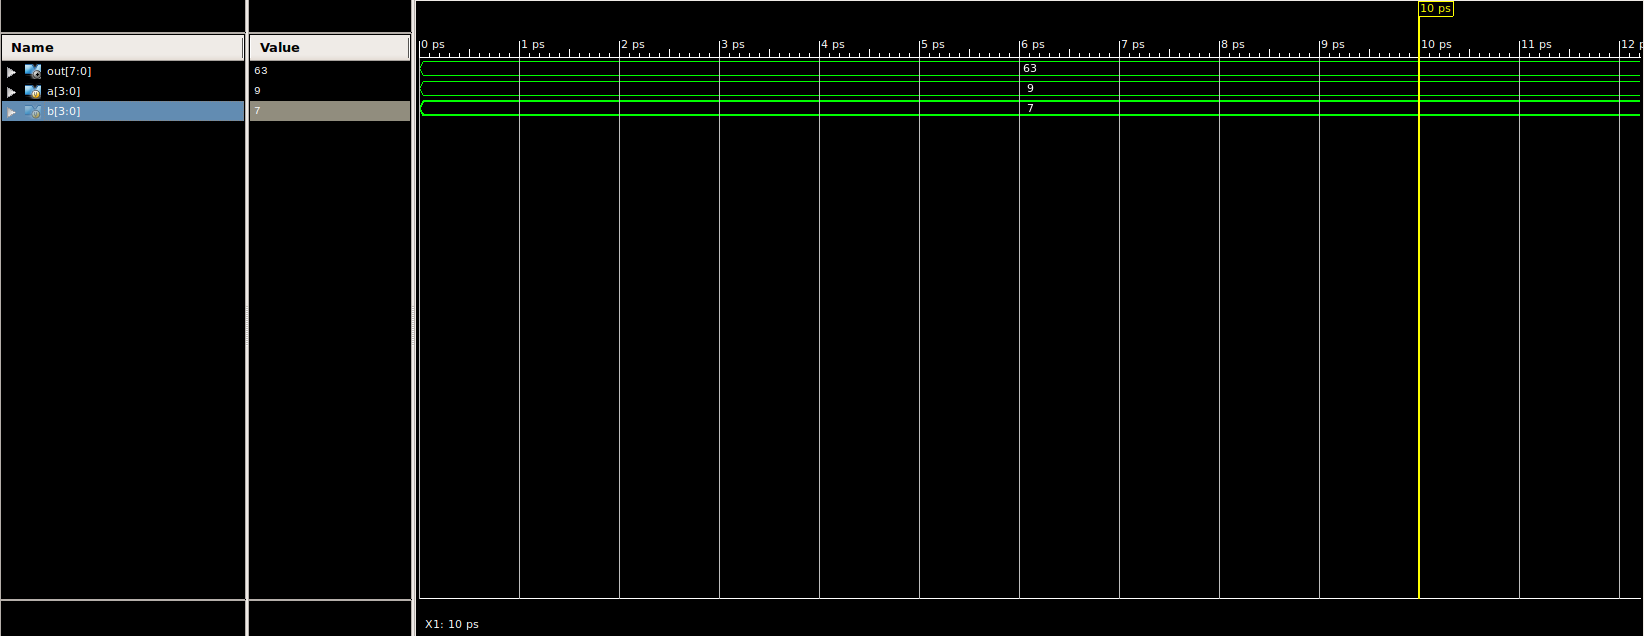
\includegraphics[width=16cm]{cs-mul-tb}
\caption{شبیه‌سازی \lr{Carry-Save Multiplier}}
\end{figure}


%\begin{latin}
%\begin{center}
%\small \begin{BVerbatim}
%NOT(0) = 1
%NOT(1) = 0
%AND(1, 1) = 1
%AND(1, 0) = 0
%AND(0, 1) = 0
%AND(0, 0) = 0
%OR(1, 1) = 1
%OR(1, 0) = 1
%OR(0, 1) = 1
%OR(0, 0) = 0
%XOR(1, 1) = 0
%XOR(1, 0) = 1
%XOR(0, 1) = 1
%XOR(0, 0) = 0
%\end{BVerbatim}
%\end{center}
%\end{latin}


%\begin{LTR}
%\lstinputlisting[caption={\rl{طراحی مدل برای دسته‌بندی دیتاست \lr{Iris}}​},label=code:iris,style=pyt]{scripts/iris.py}
%\end{LTR}

%\begin{figure}[H]
%\centering
%\includegraphics[height=9cm]{iris}
%\caption{عملکرد مدل در دسته‌بندی دیتاست \lr{Iris}}
%\label{fig:iris}
%\end{figure}
\noindent
\end{document}

